\begin{thebibliography}{1}
\bibitem{infineon_lna}
Infineon Technologies AG: \emph{BFR181W Silicon NPN RF Transistor}, Datenblatt, 2017. Online verfügbar unter: \url{https://www.infineon.com/dgdl/Infineon-BFR181W-DS-v02_00-en.pdf}

\bibitem{hf-Verstärker}
Advanced Test Equipment Corp.: \emph{What is an RF Amplifier?}, o.J. Online verfügbar unter: \url{https://www.atecorp.com/solutions/what-is-an-rf-amplifier} (zugegriffen am 17.04.2025)

\bibitem{hf-Versärker}
Wikipedia: \emph{Verstärker (Elektrotechnik)}, o.J. Online verfügbar unter: \url{https://de.wikipedia.org/wiki/Verst%C3%A4rker_(Elektrotechnik)} (zugegriffen am 17.04.2025)

\bibitem{SParrameter}
Denisowski, Paul: \emph{S-Parameter verstehen}. In: Rohde \& Schwarz GmbH \& Co. KG, o.J. Online verfügbar unter: \url{https://www.rohde-schwarz.com/de/produkte/messtechnik/essentials-test-equipment/spectrum-analyzers/s-parameter-verstehen\_257831.html\#gallery-7} (zugegriffen am 18.04.2025)
\end{thebibliography}
%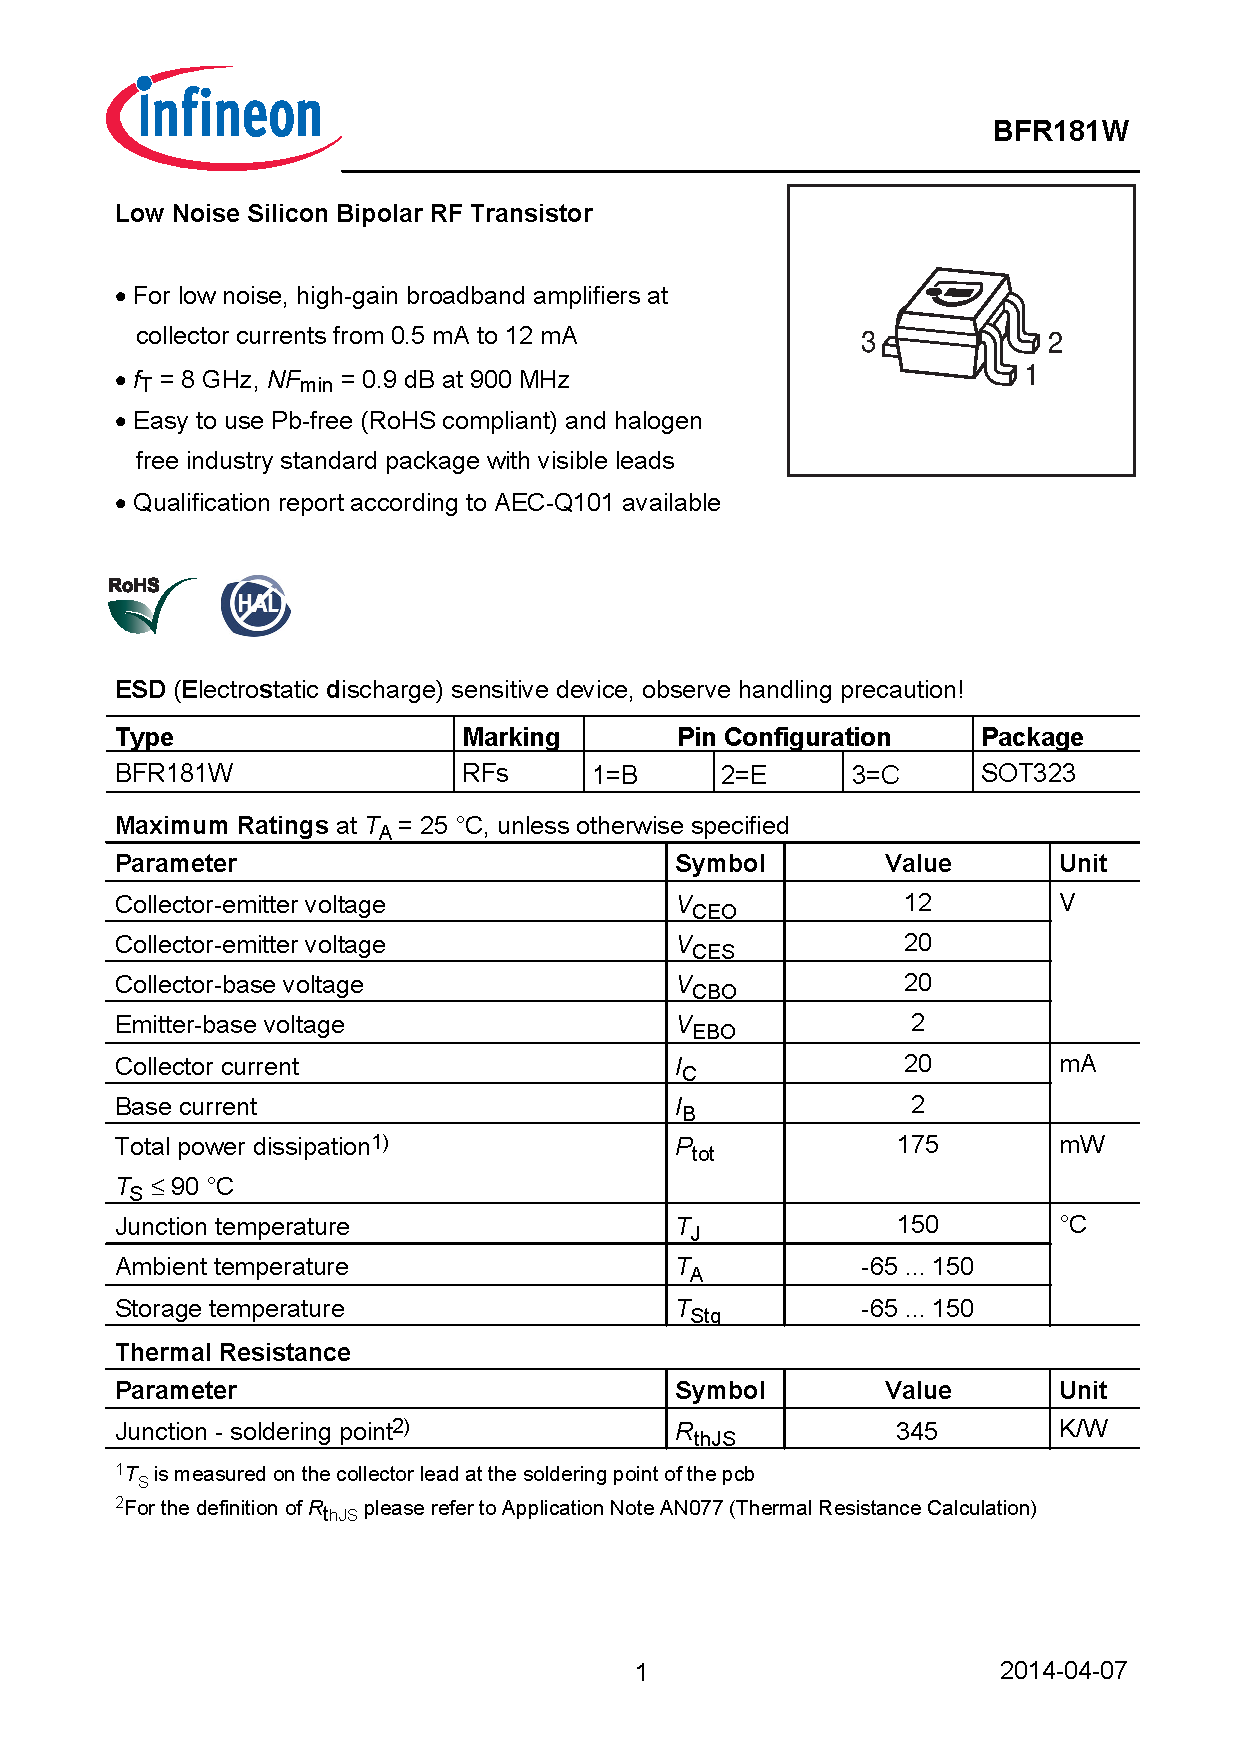
\includepdf[pages=-, pagecommand={\thispagestyle{empty}\setcounter{page}{\thepage}\rfoot{\thepage}}, fitpaper=true, offset=1.0in -1.0in]{C:/Users/Farhad/OneDrive/Desktop/Vorlage neu/GrundlagenPraktikum6G/2_Protokoll/Literature/Infineon_LNA_BFR181W-85922.pdf}
\clearpage